
\thispagestyle{empty}
\
\pagebreak

\thispagestyle{empty}
\begin{center}
	~\vfill
	
\includegraphics[scale=.4]{pictures/besm2.jpg}
	~\vfill
\end{center}
\pagebreak


\thispagestyle{empty}
\newgeometry{left=3cm,right=3cm,top=2cm}
\begin{center}
	
\includegraphics[height=3cm]{pictures/iut_logo.png} \\
	\vspace{0.5cm}
	\large\textbf{دانشگاه صنعتی اصفهان} \\ دانشکده مهندسی برق و کامپیوتر \\
	\vspace{3.5cm}
	\LARGE\textbf{ عنوان پایان‌نامه} \\
	\vspace{3.5cm}
	\large\textbf{پایان نامه کارشناسی ارشد مهندسی کامپیوتر - هوش مصنوعی و رباتیکز} \\
	\vspace{1cm}
	\Large\textbf{نام و نام خانوادگی} \\
	\vspace{2.5cm}
	\large{استاد راهنما} \\
	\vspace{0.5cm}
	\Large\textbf{دکتر استاد راهنما} \\
	\vspace{3.5cm}
	\Large\textbf{۱۴۰۱} \\
\end{center}
\restoregeometry
\pagebreak


\thispagestyle{empty}
\newgeometry{left=3cm,right=3cm,top=2cm}
\begin{center}
	
\includegraphics[height=3cm]{pictures/iut_logo.png} \\
	\vspace{0.5cm}
	\large\textbf{دانشگاه صنعتی اصفهان} \\ دانشکده مهندسی برق و کامپیوتر \\
	\vspace{2cm}
	\LARGE{پایان نامه کارشناسی ارشد مهندسی کامپیوتر - هوش مصنوعی و رباتیکز\\آقای نام و نام خانوادگی تحت عنوان} \\
\end{center}
\vspace{4cm}
\begin{flushright}
	\Large\textbf{عنوان پایان‌نامه} \\
	\vspace{2.5cm}
	\normalsize\setstretch{2.5}{
		در تاریخ ۱۴۰۱/۶/۱۶ توسط کمیته تخصصی زیر مورد بررسی و تصویب نهایی قرار گرفت:
		\begin{multicols}{2}
			۱. استاد راهنمای پایان‌نامه\\\columnbreak دکتر استاد راهنما
		\end{multicols}
		\begin{multicols}{2}
			۲. استاد داور\\\columnbreak دکتر استاد داور ۱
		\end{multicols}
		\begin{multicols}{2}
			۳. استاد داور\\\columnbreak دکتر استاد داور ۲
		\end{multicols}
		\begin{multicols}{2}
			سرپرست تحصیلات تکمیلی دانشکده\\\columnbreak دکتر سرپرست ت.ت.
		\end{multicols}
	}
\end{flushright}
\restoregeometry
\pagebreak


\thispagestyle{empty}
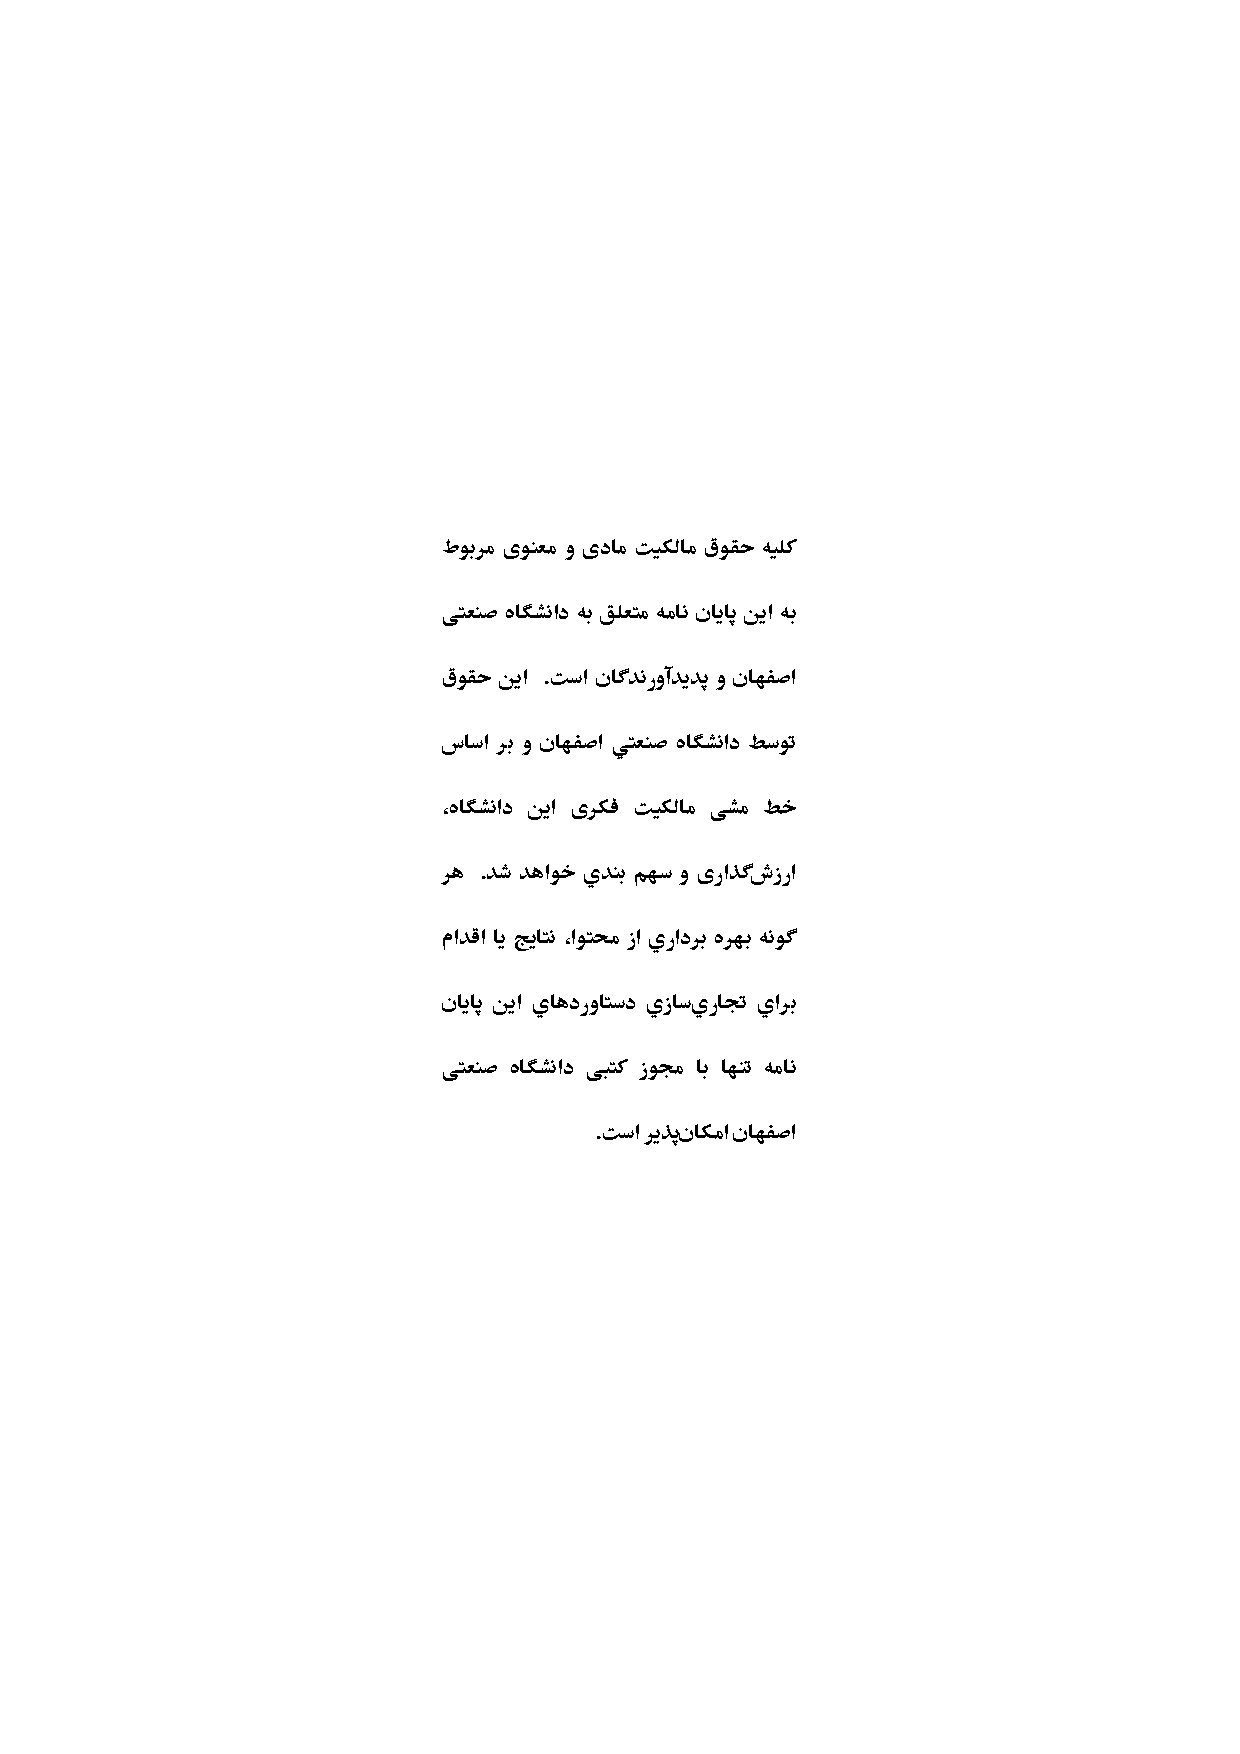
\includepdf[pages=-]{contents/copywrite.pdf}
\restoregeometry
\pagebreak


\thispagestyle{empty}
\vspace*{3cm}
{\large
	\textbf{تقدیم به آن‌هایی که دوستشان دارید}\\
	
	\textbf{که کمک کردند}
}
\restoregeometry
\pagebreak
